\chapter{Control Unit}
\label{Control Unit}
The Control Unit is an Hardwired Control Unit and controls the Datapath generating the proper controlword based on current instruction in the proper clock cycle. It is divided in different parts:

\begin{figure}[h!]
	\centering
	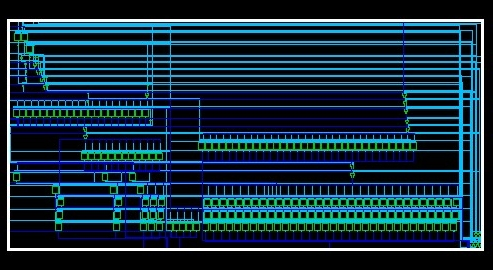
\includegraphics[width=\textwidth]{chapters/figures/ControlUnit_highlevel.jpg} 
	\caption{Synthetized Control Unit}
	\label{fig:cu}  % here is the figure label
	\end{figure}

\begin{enumerate} 
    \item Look-Up Table: it contains all the control words linked to the instrunctions
    \item Three processes that work one after the other:
    \begin{enumerate}
    \item The first one takes the main input of CU (IR\_In) and consider the relative opcode and func of the instruction which are used by the second process.
    \item The second one takes the opcode and func of the first process (checking if RTYPE,ITYPE,JTYPE) and use them to take the correct control word from the look-up table.
    \item The last one works to pipeline the control words in the right way (as an Hardwired Control Unit do) and there is also the pipeline of the instructions that it is used for the Hazard Unit.This process, also, takes as inputs the three hazard signals from the HU to flush the pipeline putting NOP in the decode stage and execute stage for branch hazard or putting NOP in decode stage for jump untill the new PC or putting NOP in execute stage and maintaining the same control word (and istruction)in the decode stage for raw hazard.The flush of the pipeline depends on where the hazard is taken (specified in the HU chapter), it lasts one or more cycles. 
    \end{enumerate}
\end{enumerate}
\subsection{Control Word}
The main job of the Control Unit is to generate the right control word using the look-up table. Each control word is saved in the file "INSTR\_CODES.vhd" with all the opcode and func of the instructions.
The bits are divided for Decode Unit, Execution Unit, Memory Unit, Writeback Unit and they are pipelined during the cycles to be used in the correct moment of the pipeline to activate the useful components of the datapath.

